\section*{Аннотация}
\addcontentsline{toc}{section}{Аннотация}

Холодные нейтральные атомы в массивах оптических пинцетов являются лидирующей платформой для реализации квантового компьютера. Для практического использования такого компьютера важно уметь выполнять однокубитные и многокубитные логические операции с высокой точностью. В работе исследуются подходы к улучшению точности однокубитных логических операций с рамановским двухфотонным возбуждением и двухкубитных логических операций, реализуемых с помощью эффекта ридберговской блокады. Проводится моделирование основных источников ошибок, включающих в себя тепловое движение атома в оптическом пинцете, спонтанный распад из промежуточного состояния, фазовые шумы лазера, ошибки приготовления и измерения состояния. Параметры модели экспериментально измеряются, что позволяет запускать моделирование без свободных параметров. Также экспериментально демонстрируется повышение достоверности логических операций за счёт использования flat-top пучков и последовательностей импульсов. 

\vspace{4em}
\begin{figure}[ht]
	\centering
	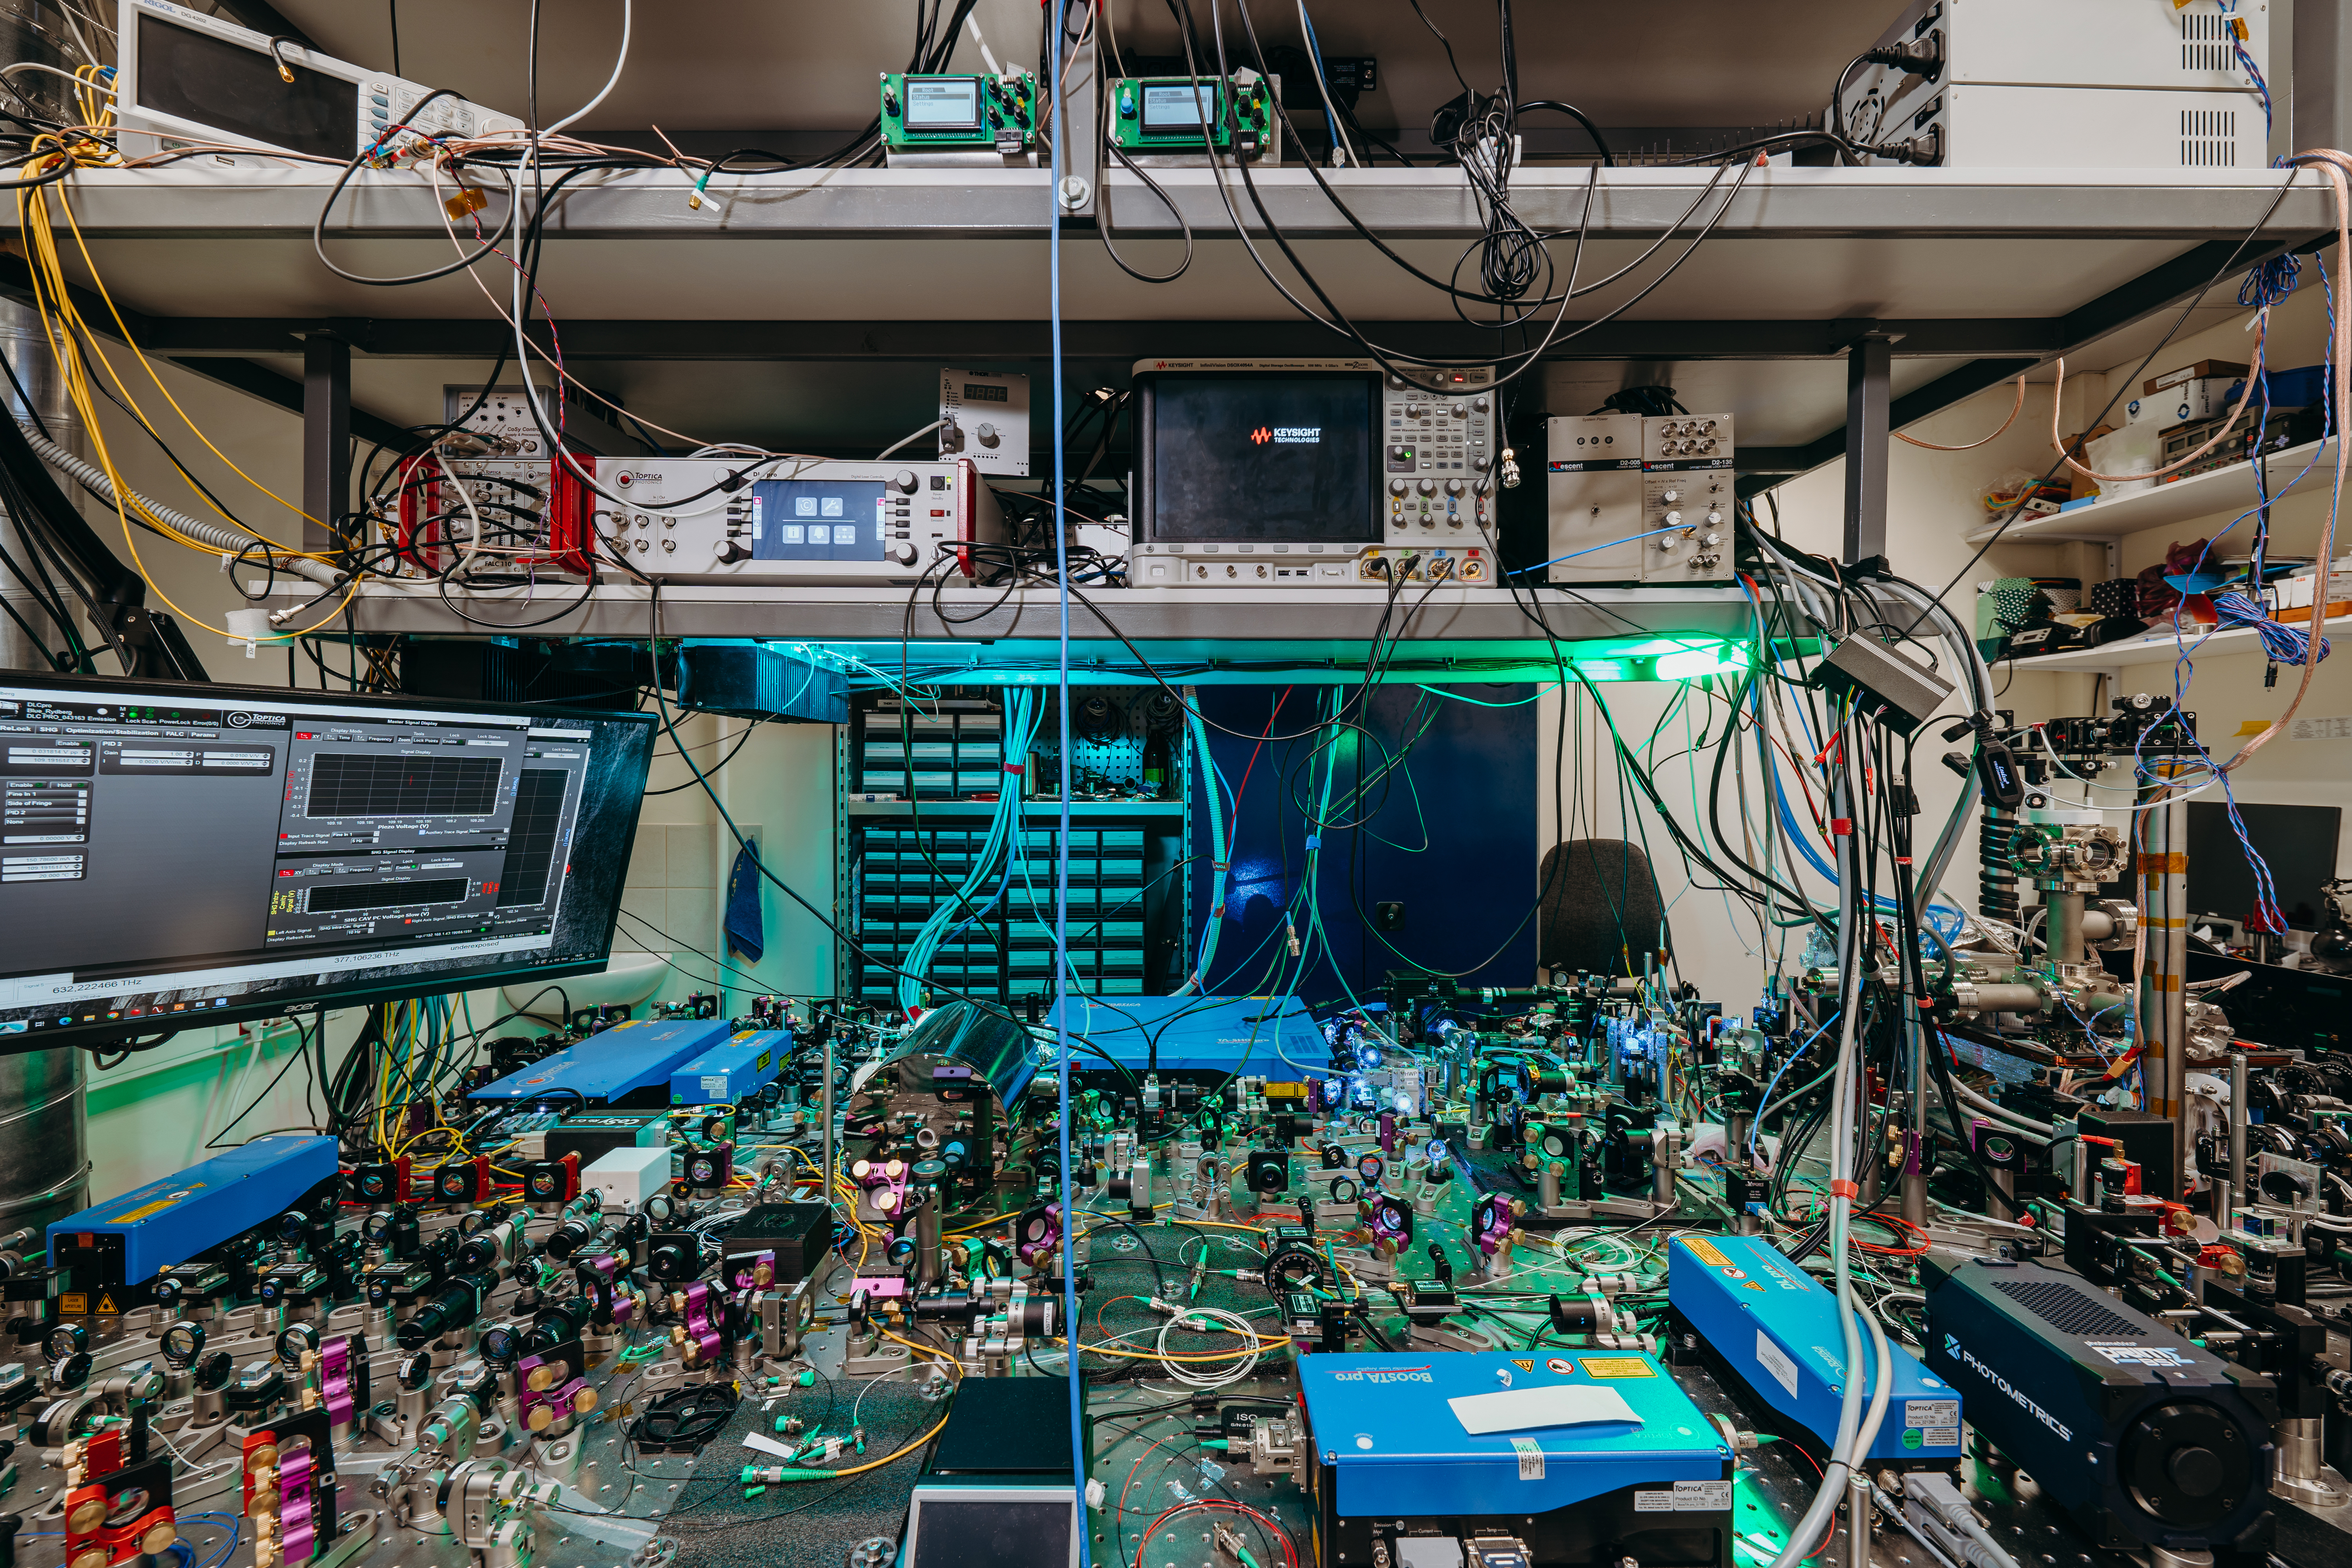
\includegraphics[width=1.0\textwidth]{images/QuantumComputer.jpg}
	\caption{Квантовый компьютер на холодных нейтральных атомах $^{87}\text{Rb}$ лаборатории ``Атомных и оптических квантовых вычислений''.}
\end{figure}

\newpage